\documentclass[tikz,border=3mm]{standalone}
\usepackage[normalem]{ulem}
\usepackage{tikz, shapepar}
\usepackage{shapepar}
\usetikzlibrary{mindmap, trees}
\usetikzlibrary{positioning,fit,calc,backgrounds}
%\tikzset{block/.style={draw,thick,text width=3cm,minimum height=2cm,align=center},
%         line/.style={-latex}
%}
%\makeatletter
%\def\ruwave{\bgroup \markoverwith{\lower7\p@\hbox{\textcolor{red}{\sixly \char116}}}\ULon}
%\font\sixly=lasy6
%\makeatother


\begin{document}
	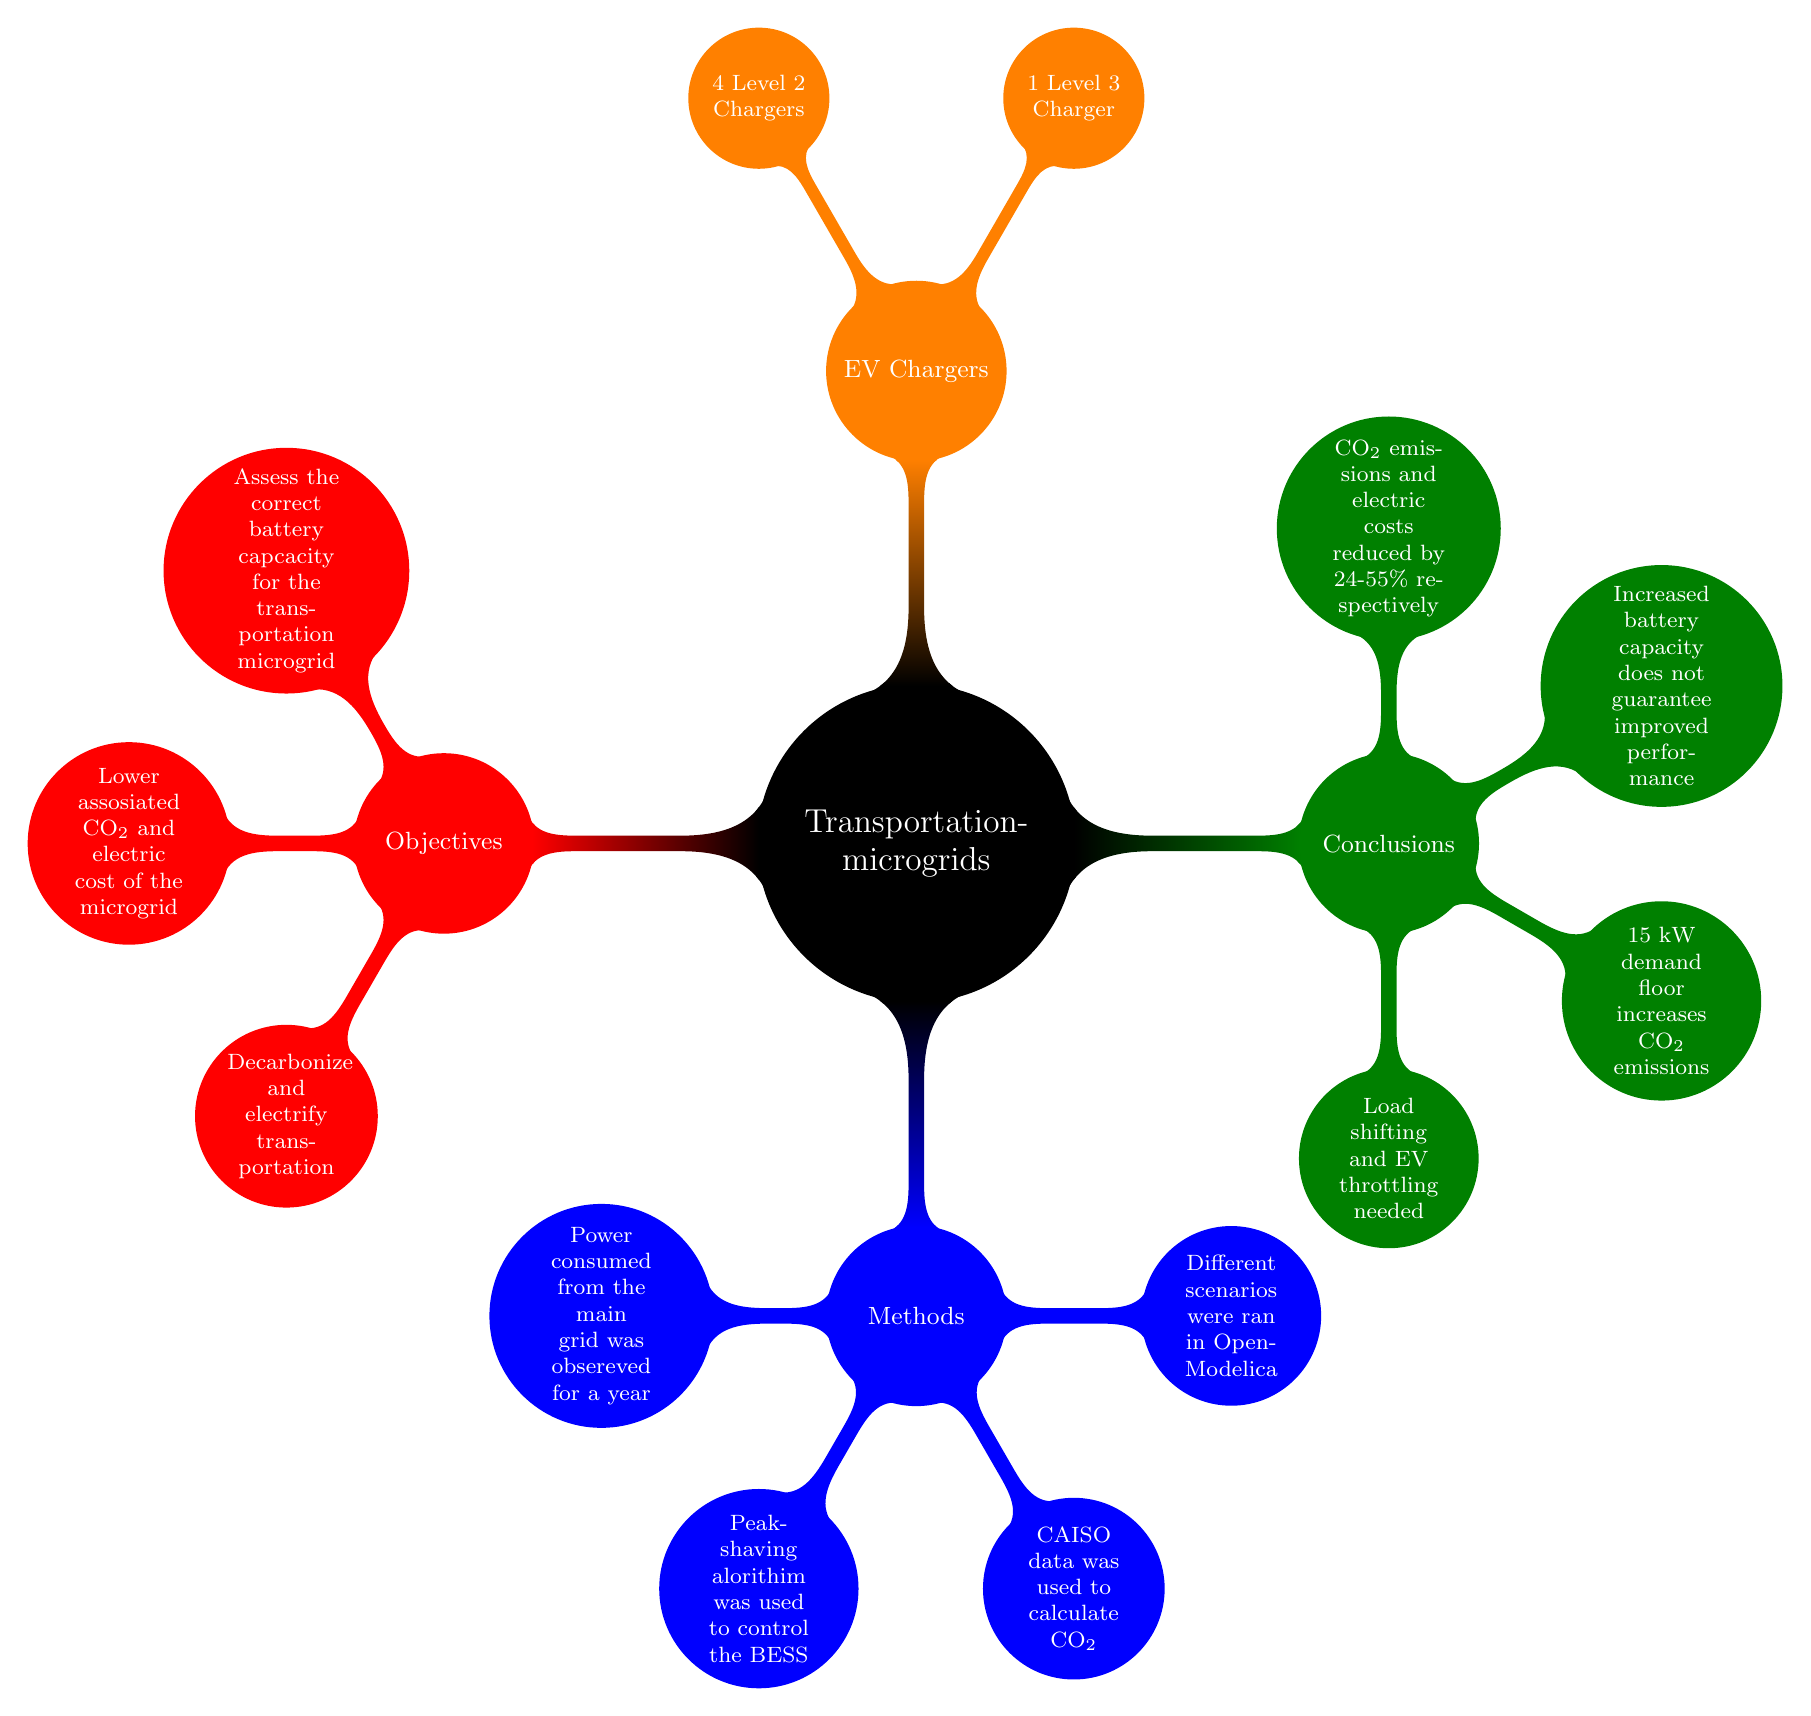
\begin{tikzpicture}
%	\path[mindmap,concept color=black,text=white]
\path[
mindmap,
concept color=black,
text=white,
grow cyclic,
segment length=20cm,
level 1/.append style={level distance=6cm,sibling angle=90},
level 2/.append style={level distance=4cm},
]
	node[concept] {Transportation-microgrids}
	[clockwise from=0]
	% note that `sibling angle' can only be defined in
	% `level 1 concept/.append style={}'
	child[concept color=green!50!black] {
		node[concept] {Conclusions}
		[clockwise from=90]
		child { node[concept] { CO\textsubscript{2} emissions and electric costs reduced by 24-55\% respectively } }
		child { node[concept] { Increased battery capacity does not guarantee improved performance} }
		child { node[concept] { 15 kW demand floor increases CO\textsubscript{2} emissions} }
		child { node[concept] { Load shifting and EV throttling needed } } 
	}
	% note that the `concept color' is passed to the `child'(!)
	child[concept color=blue] {
		node[concept] {Methods}
		[clockwise from=-0]
		child { node[concept] {Different scenarios were ran in OpenModelica} }
		child { node[concept] {CAISO data was used to calculate CO\textsubscript{2}} }
		child { node[concept] {Peak-shaving alorithim was used to control the BESS} }
		child { node[concept] {Power consumed from the main grid was obsereved for a year} }
	}
	child[concept color=red] { node[concept] {Objectives} 
	[clockwise from=-120
	]
	child { node[concept] {Decarbonize and electrify transportation} }
	child { node[concept] {Lower assosiated CO\textsubscript{2} and electric cost of the microgrid} }
	child { node[concept] {Assess the correct battery capcacity for the transportation microgrid} }
	}
	child[concept color=orange] { 
	node[concept] {EV Chargers}
	[clockwise from=-240]
	child { node[concept] {4 Level 2 Chargers} }
	child { node[concept] {1 Level 3 Charger} }
	};
	\end{tikzpicture}
\end{document}